% Chapter Template

\chapter{Conclusiones} % Main chapter title

\label{Chapter5} % Change X to a consecutive number; for referencing this chapter elsewhere, use \ref{ChapterX}


%----------------------------------------------------------------------------------------

%----------------------------------------------------------------------------------------
%	SECTION 1
%----------------------------------------------------------------------------------------
En este capítulo se destacan los principales aportes al trabajo realizado, se evalúa el cumplimiento de los requerimientos y se destacan los conocimientos aplicados.
\section{Conclusiones generales del trabajo realizado}


Los principales resultados del trabajo realizado son los siguientes:

\begin{itemize}
    \item Se logró construir un prototipo de hardware principal y un prototipo por cada uno de los dos módulos de comunicación de acuerdo al objetivo establecido.
    \item A partir de los resultados presentados en el capitulo \ref{Chapter4} se puede afirmar que no es necesario realizarle una sintonización a la antena externa que lleva el dispositivo, debido a que cumple con los parámetros teóricos y empíricos mencionados en la sección \ref{subseccionAntena}
\end{itemize}


\begin{itemize}
    \item Se concluye además de acuerdo a las mediciones realizadas que el modulo Sigfox consume menos energía en modo normal y en bajo consumo que el modulo LoRaWAN. esto permite que pueda ser útil en muchas aplicaciones donde lo primordial es la durabilidad de la batería del dispositivo.
    \item El consumo de los dispositivos se puede ver afectado por un ensamble defectuoso, como exceso de soldadura o soldaduras en frió. Se debe garantizar que los pines sobrantes en el microcontrolador se coloque como entradas analógicas (alta impedancia) y también se deben garantizar los niveles lógicos de las entradas digitales. Cabe aclarar que estas son conclusiones que se dan de acuerdo a la experiencia con el manejo de dispositivos de bajo consumo y el desarrollo del presente trabajo. Sin embargo se debe siempre acudir a la hoja de datos y recomendaciones del fabricante.
\end{itemize}

\begin{itemize}
    \item Para decidir cual de las dos tecnologías (Sigfox o LoRa) a usarse debe analizar el caso de uso y la región, por que por ejemplo en Colombia  no hay un gran proveedor de la red LoRa como si lo tiene Sigfox. Sin embargo hay quienes prefieren montar el servidor y la red con LoRa ellos mismos y hay otras personas que prefieren tener todo a la mano como se lo brinda Sigfox. En otros países donde la red loRa tiene mas despliegue, quizás Sigfox no sea la mejor opción, debido a que en LoRa se puede tener una mejor transferencia de datos y mejor confirmación con mensajes de subida. En los mensajes de bajada no tiene la restricción de 120 mensajes mensuales como si lo tiene Sigfox.
    \item De acuerdo a los resultados de las transmisiones con LoRaWAN, se tiene que de los mensajes transmitidos solo el 3.85 \% de ellos llegaron al servidor, esto debido a que el gateway que se tenía disponible era de un solo canal y no era el optimo para este uso.
\end{itemize}


\subsection{Cumplimiento de los requerimientos}

Todos los requerimientos se implementaron de forma exitosa. Sin embargo de acuerdo a las sugerencias del director se decidió enfocar el proyecto una de las dos tecnologías, en este caso Sigfox debido a que se presentaron inconvenientes en la adquisición del gateway LoRa, sin embargo se lograron realizar algunas transmisiones con un gateway LoRa de un solo canal obtenido a ultimo momento.

Cabe mencionar que el inconveniente mas relevante fue el no poder tener un gateway apropiado en el momento necesario.

\subsection{Conocimientos utilizados}
Para el desarrollo de este trabajo se utilizaron los siguientes conocimientos.

\begin{itemize}
\item Programación de microprocesadores: se aprovecha la experiencia adquirida en lenguaje C en microcontroladores con arquitecturas de 32 bits y se aplica a otro microcontroladores como lo es STM32.
\item Gestión de proyectos: El aporte de esta asignatura contribuyo considerablemente en el desarrollo de un plan de trabajo claro y organizado, permitiendo que el desarrollo del proyecto se ejecutara de la mejor manera.
\item Protocolos de comunicación en sistemas embebidos: Se aplicaron los conocimientos para la programación de los periféricos I2C y UART. También se aplicaron los conocimientos de desarrollo de manejadores de dispositivos en los drivers del modulo Sigfox y LoRaWAN.
\item Sistemas Operativos de Tiempo Real (I y II) : Con estas asignaturas se desarrollo una mejor perspectiva de los sistemas concurrentes en sistemas embebidos y fue muy útil en el desarrollo del firmware del proyecto, ya que se uso un sistema operativo cooperativo .
\end{itemize}

También se adquirieron conocimientos en:
\begin{itemize}
    \item Configuración de módems.
    \item Trasmisión de datos a plataformas integradoras pagas y \textit{open source}.
    \item Control de versiones.
    \item Test de pruebas unitarias.
\end{itemize}

Y se aplicaron conocimientos previamente adquiridos como:
\begin{itemize}
    \item \textit{Testing} y control de calidad en los circuitos.
    \item Diseño electrónico y de PCB.
    \item Diseño de antenas.
    \item Sintonización de antenas.
    \item Desarrollo de firmware y manejadores de dispositivos orientado a objetos.
\end{itemize}


%----------------------------------------------------------------------------------------
%	SECTION 2
%----------------------------------------------------------------------------------------
\section{Trabajo futuro}

Para el futuro del proyecto se propone trabajar con las tecnologías NB-IoT, CAT-M1 ó GSM. Hay algunos módulos como el BG96 de la marca Quectel que incorpora estas dos tecnologías de comunicación, 2G y GPS. Sin embargo,por costos también se puede trabajar estas tecnologías en módulos individuales, ya que el dispositivo de adquisición de datos permite acoplarlo fácilmente, simplemente diseñando una tarjeta con el conector adecuado y que se pueda comunicar por UART o I2C. 


% En la figura \ref{fig:gsm1} y \ref{fig:gsm} se puede observar el módulo UC20 fabricado por la empresa Quectel, este trabaja bajo la red 2G, 3G y tiene GPS interno.


% \begin{figure}[H]
% 	\centering
% 	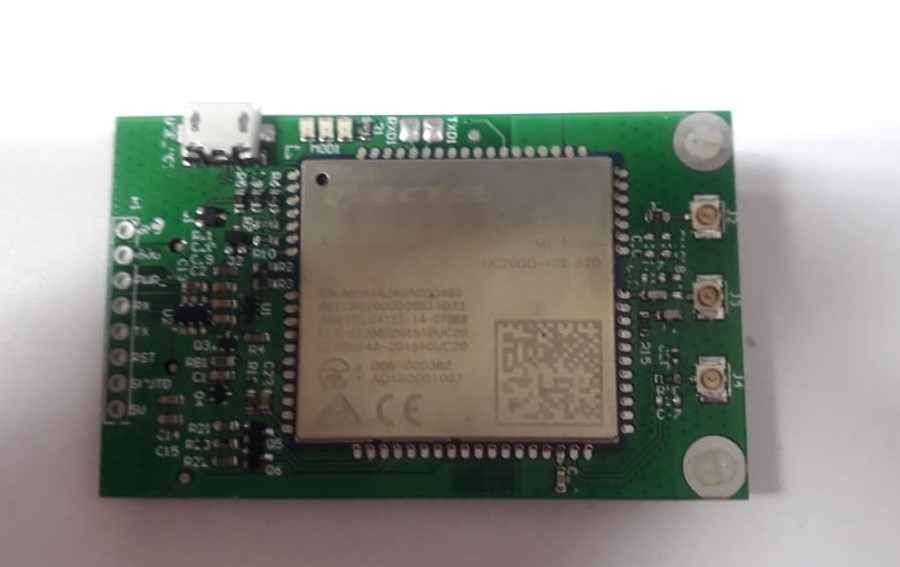
\includegraphics[scale=.45]{./Figures/gsm1.jpeg}
% 	\caption{Vista frontal del módulo 2G y 3G insertable.}
% 	\label{fig:gsm1}
% \end{figure}

% \begin{figure}[H]
% 	\centering
% 	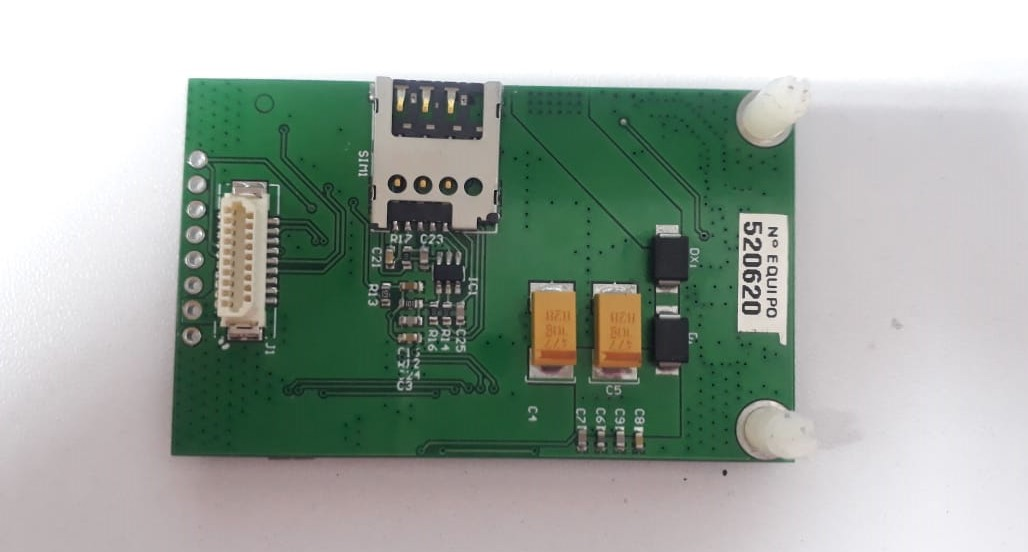
\includegraphics[scale=.45]{./Figures/gsm.jpeg}
% 	\caption{Vista posterior del módulo 2G y 3G insertable.}
% 	\label{fig:gsm}
% \end{figure}
